\section{Supplementary material}

\subsection{Synthetic MJP}

  \begin{figure}%[b]
  \centering
  \begin{minipage}[hp]{0.45\linewidth}
  \centering
    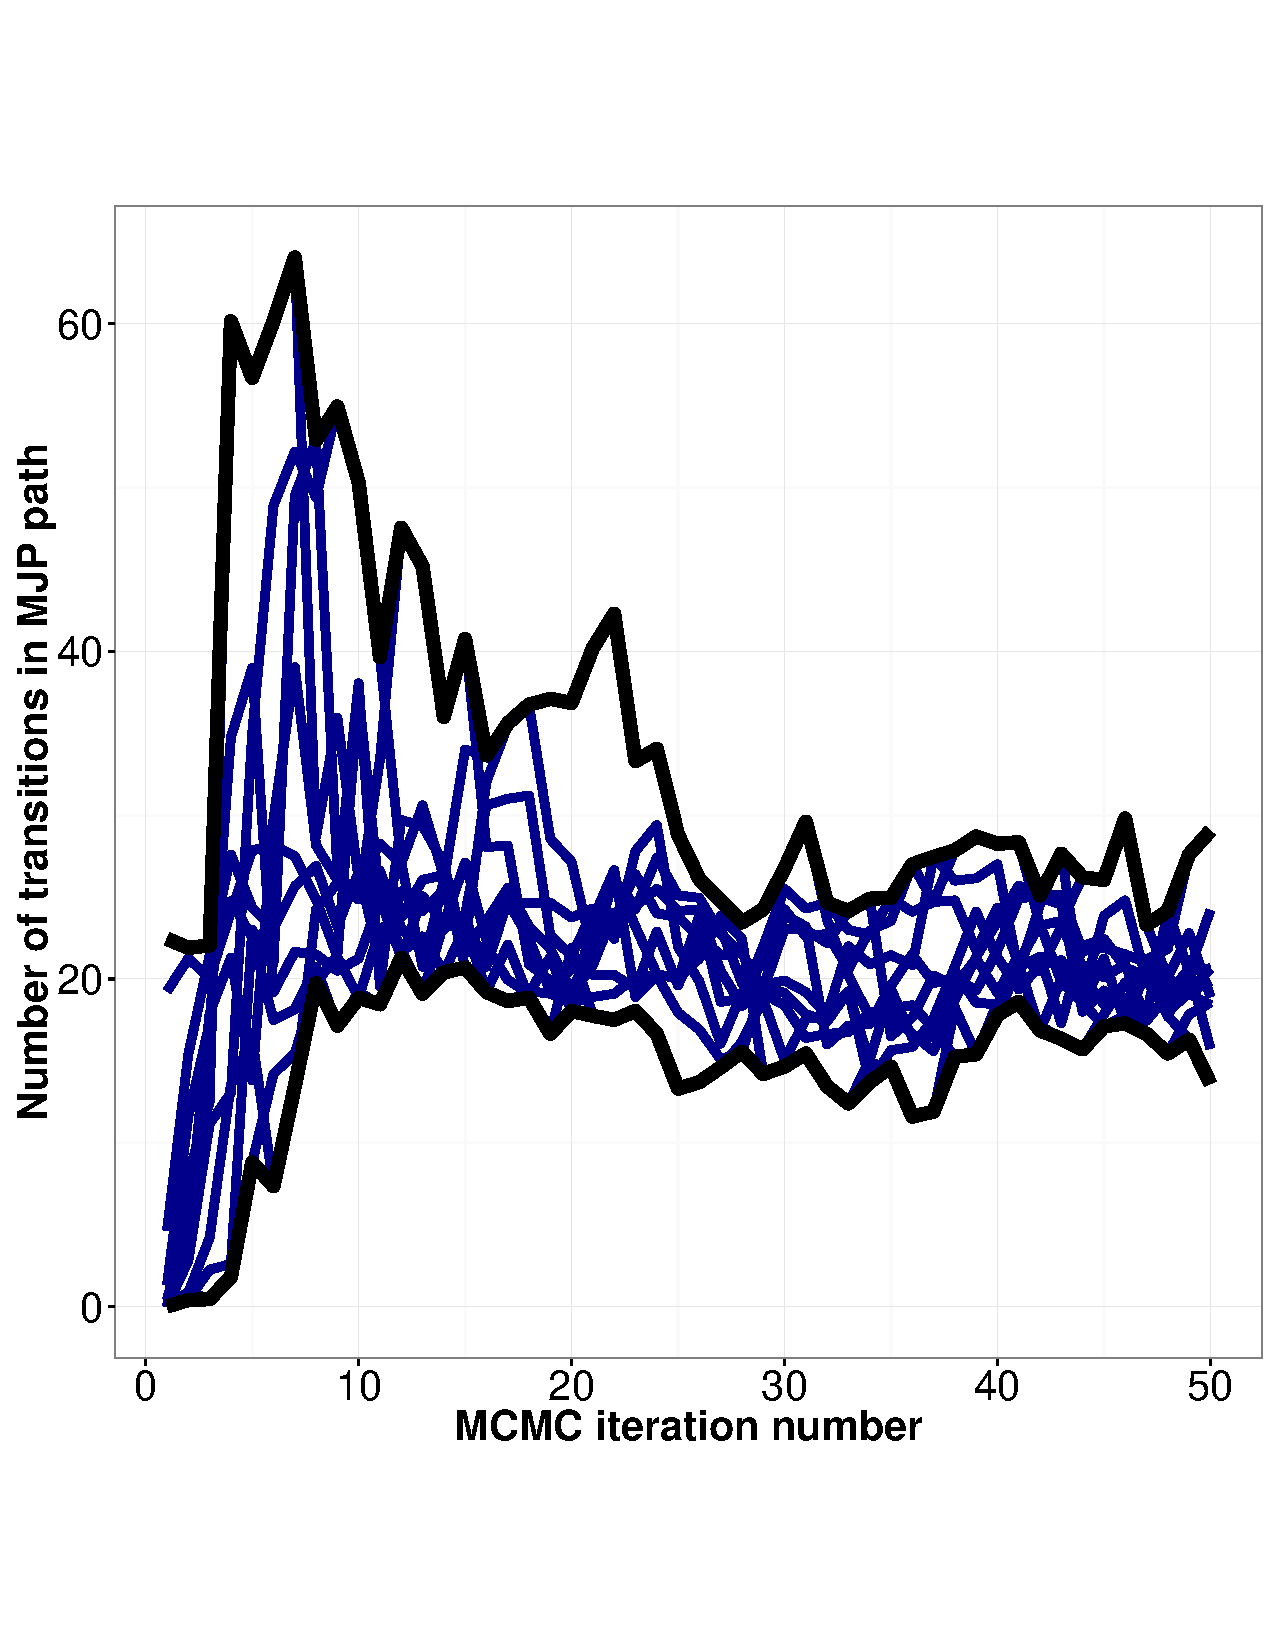
\includegraphics [width=0.90\textwidth, angle=0]{figs/exp3_k2_path_transition.pdf}
      \end{minipage}
    \caption{Trace plot of the number of MJP transitions for different initializatoins.}
	\label{fig:Transition_exp}
  \end{figure}

  \begin{figure}%[b]
  \centering
  \begin{minipage}[hp]{0.45\linewidth}
  \centering
    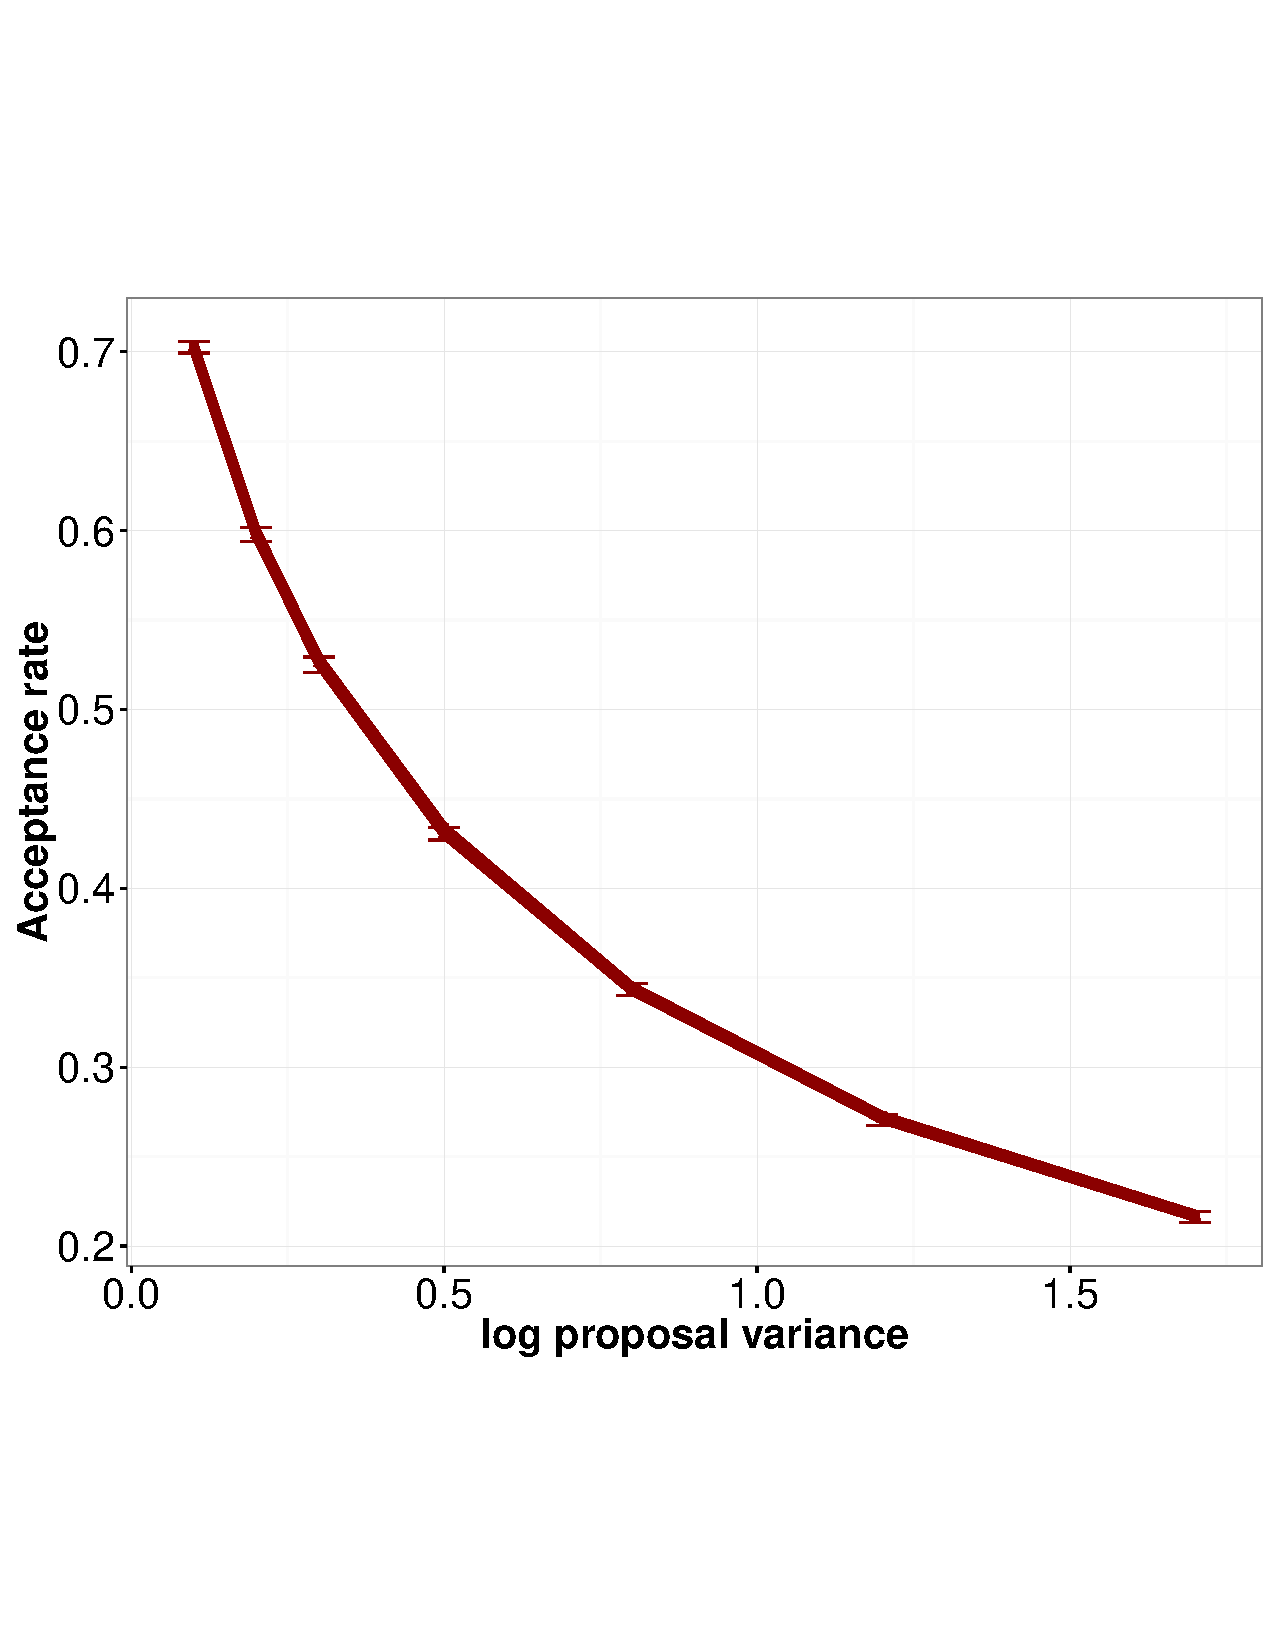
\includegraphics [width=0.90\textwidth, angle=0]{figs/acc_rate_exp_d3.pdf}
      \end{minipage}
    \caption{Acceptance rate for exp model (dim 3)}
	\label{fig:acc_exp}
  \end{figure}

Figure~\ref{fig:acc_exp} plots ESS plots the overall  acceptance rate against 
the log variance of the proposal kernel per run for dimension $3$. 



  
    \begin{figure}%[b]
  \centering
  \begin{minipage}[hp]{0.45\linewidth}
  \centering
    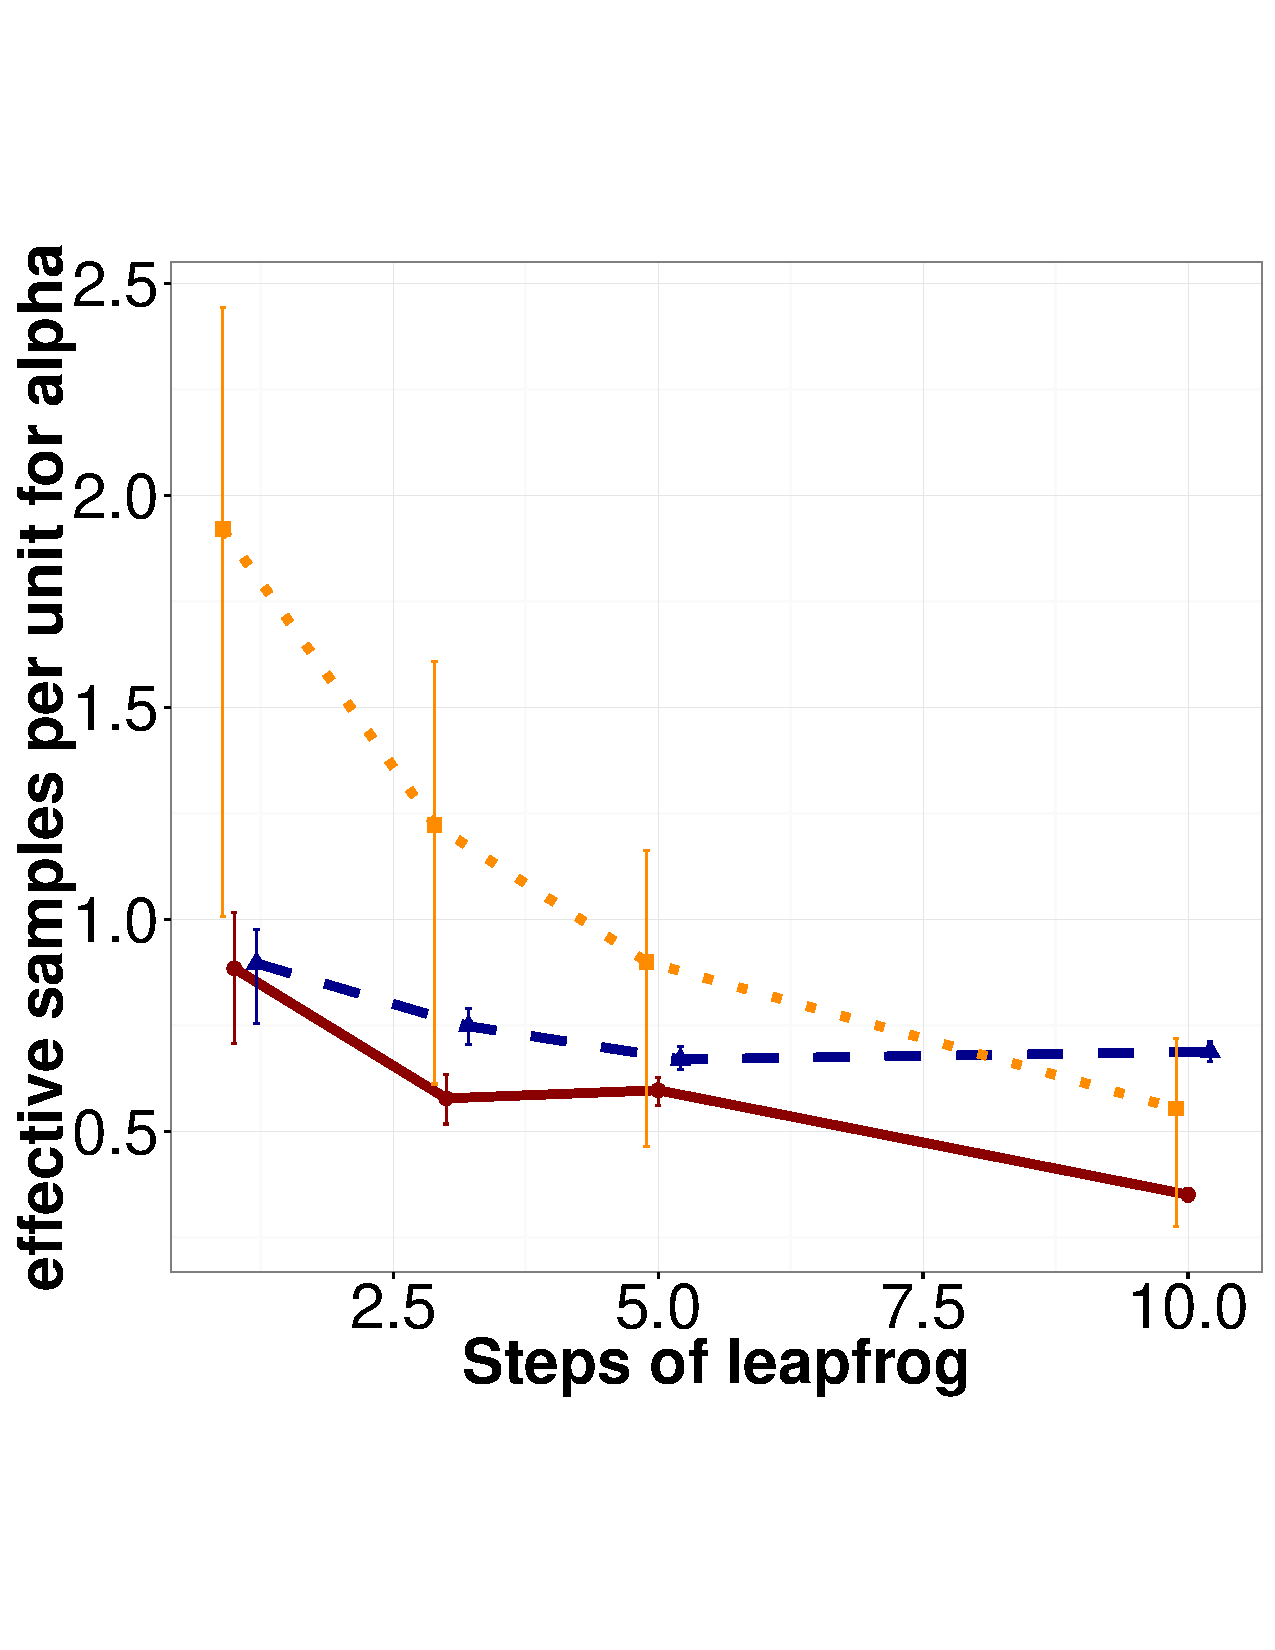
\includegraphics [width=0.90\textwidth, angle=0]{figs/h_alpha.pdf}
      \end{minipage}
  \begin{minipage}[hp]{0.45\linewidth}
  \centering
    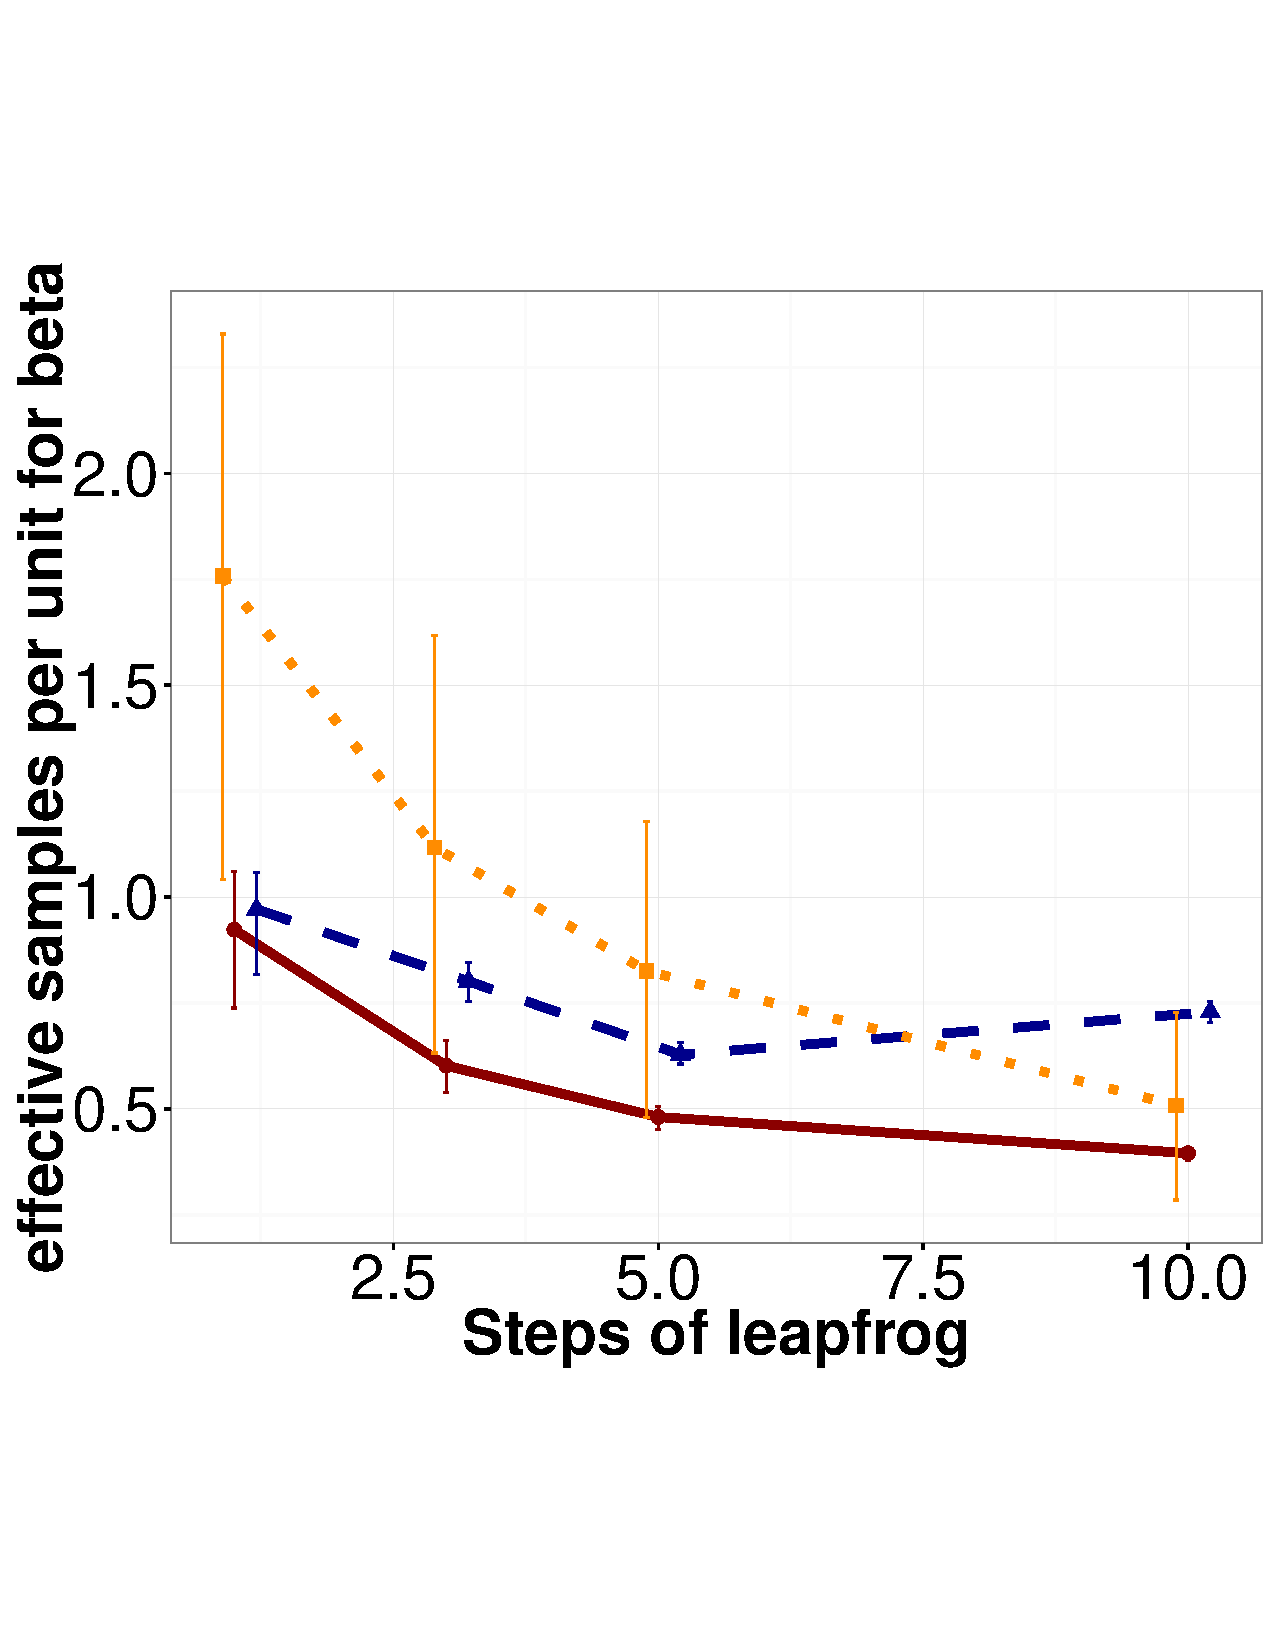
\includegraphics [width=0.90\textwidth, angle=0]{figs/h_beta.pdf}
      \end{minipage}
    \caption{HMC for dim 3}
    \label{fig:HMC_DIM_3}
  \end{figure}
In Figure~\ref{fig:HMC_DIM_3}, we plot the ESS per unit time as we change the 
number of leapfrog jumps in Hamiltonian MCMC for dimension $3$. We consider 
three different step size for leapfrog step($s = 0.02, 0.05, 0.1$). We 
use the same data for our previous experiment for the case when dimension $3$. 
We set the $m_1 = m_2 = 1.0$. Because using FFBS to explore the gradient needs 
a lot of computation, it does not work so well.\\

  \begin{figure}%[b]
  \centering
  \begin{minipage}[!hp]{0.45\linewidth}
  \centering
    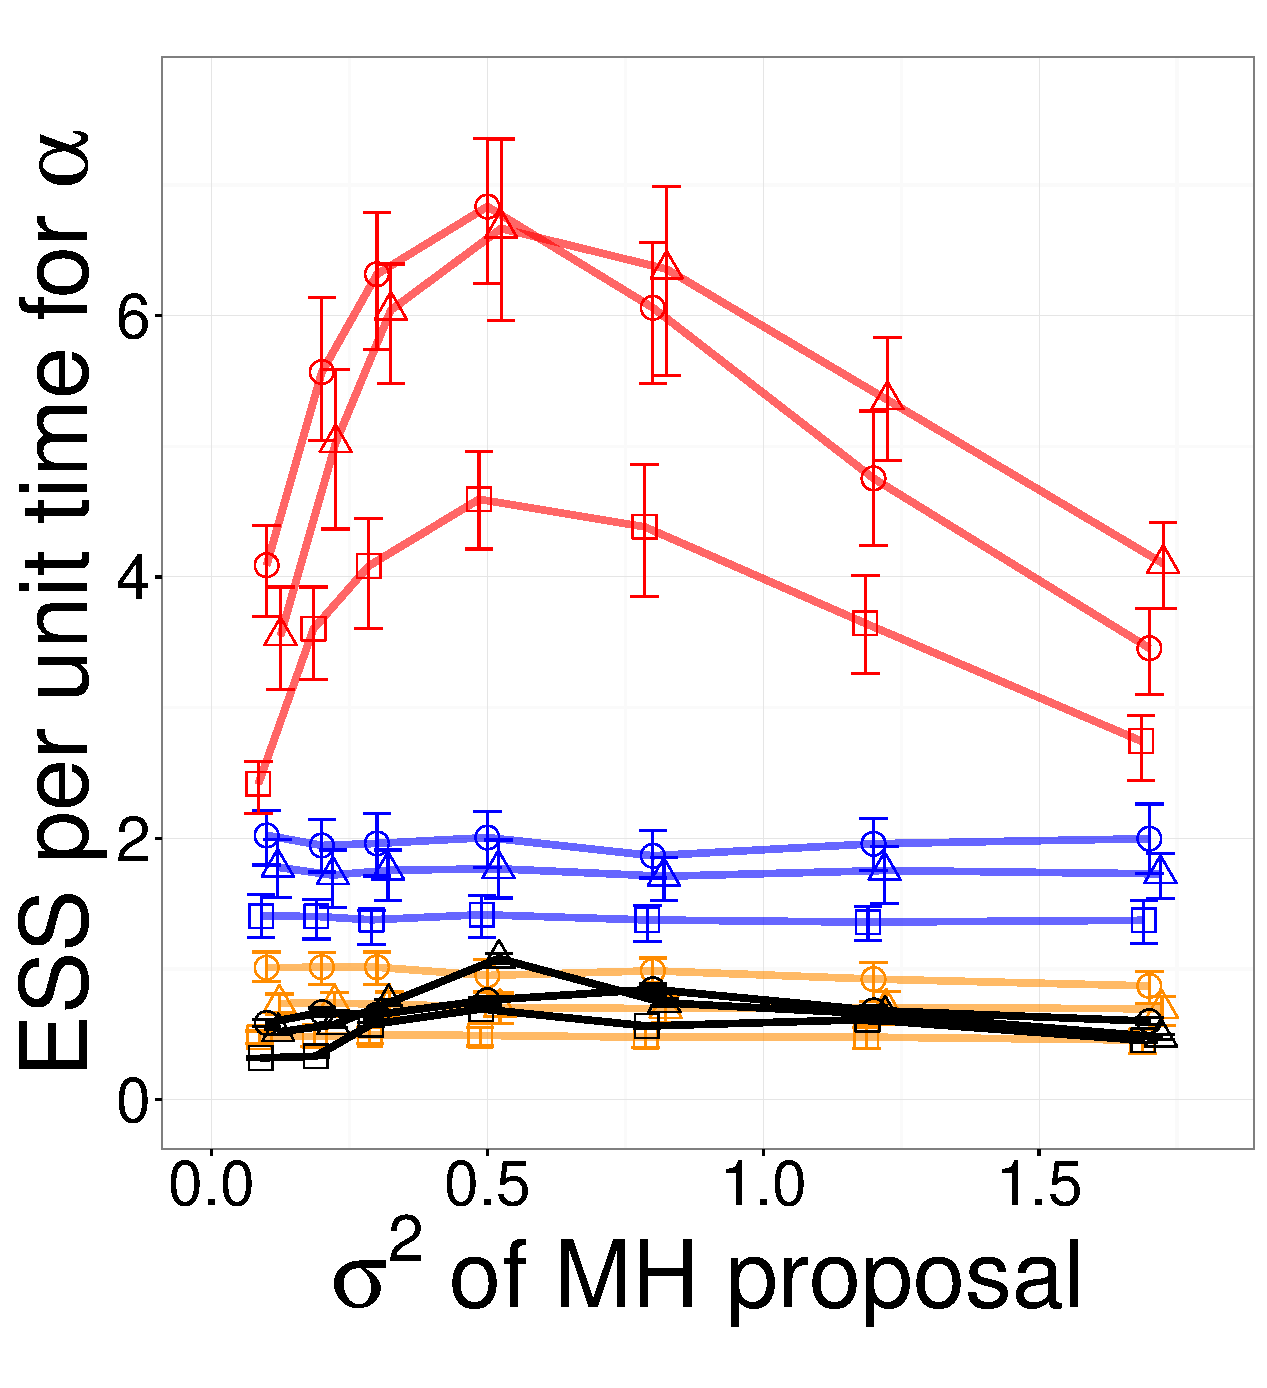
\includegraphics [width=0.90\textwidth, angle=0]{figs/exp_5_alpha.pdf}
      \end{minipage}
  \begin{minipage}[hp]{0.45\linewidth}
  \centering
    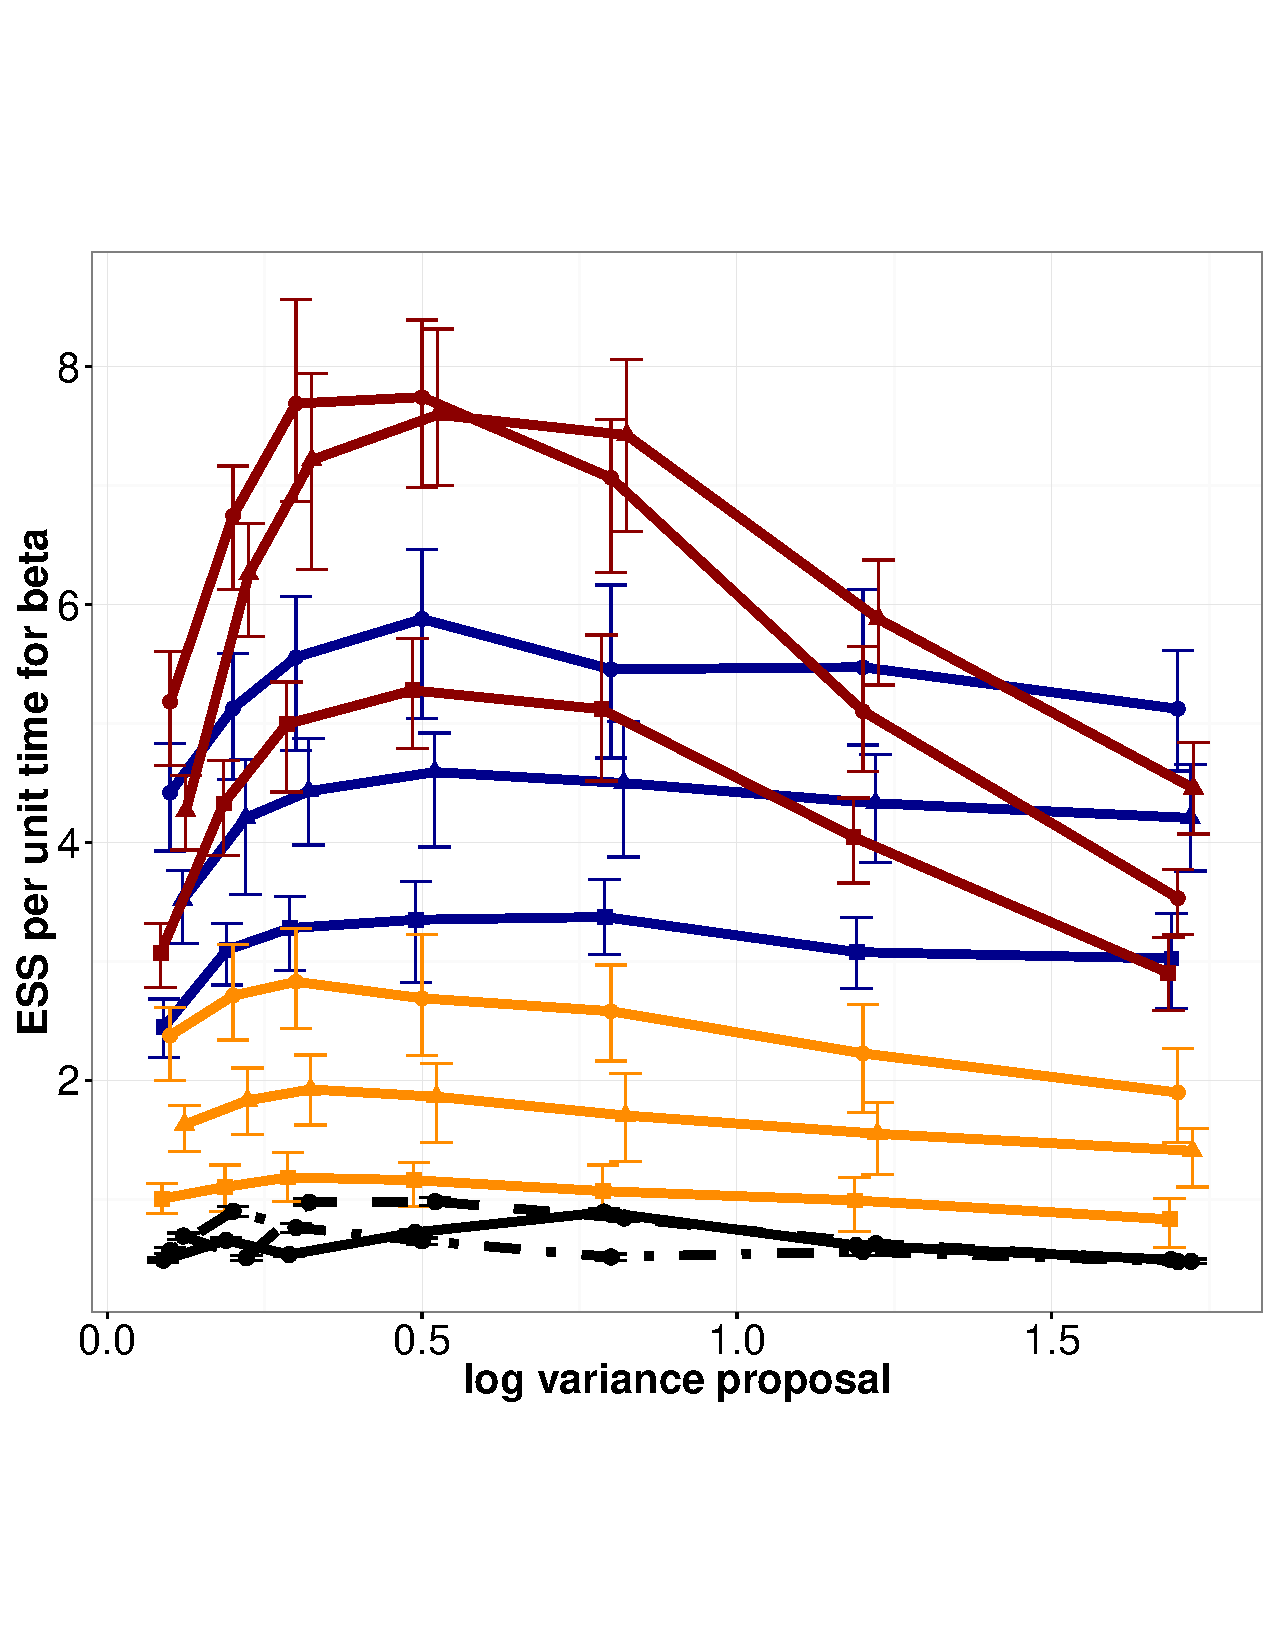
\includegraphics [width=0.90\textwidth, angle=0]{figs/exp_5_beta.pdf}
    \vspace{-0 in}
  \end{minipage}
    \caption{ESS/sec for exp model (dim 5). The left is for $\alpha$, and the right is for $\beta$.}
     \label{fig:ESS_EXP_D5}
  \end{figure}

\subsection{Immigration model with capacity}
\begin{figure}
  \begin{minipage}[hp]{0.45\linewidth}
  \centering
    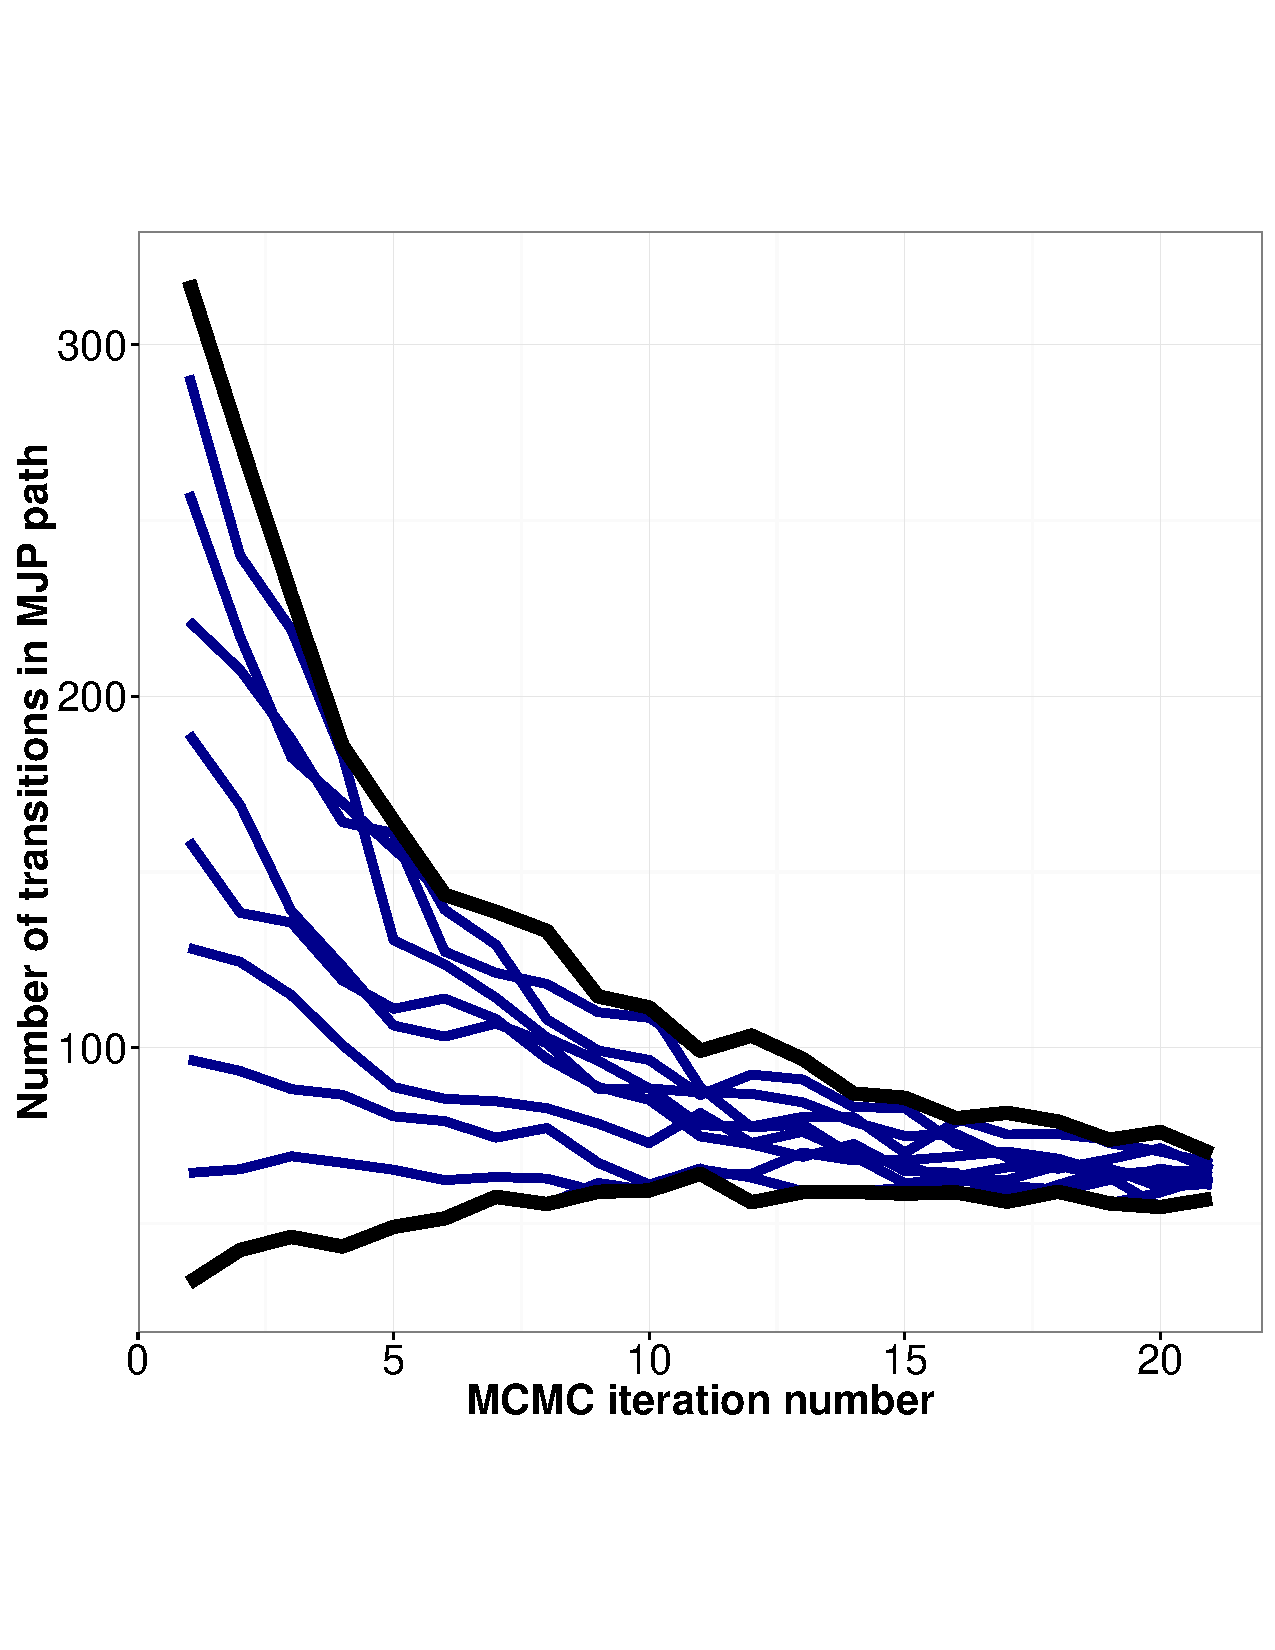
\includegraphics [width=0.90\textwidth, angle=0]{figs/q3_k2_path_transition.pdf}
    \vspace{-0 in}
    \caption{Trace plot of the number of MJP transitions for different initializatoins for immigration model.}
     \label{fig:ESS_Q_TRANSITION}
  \end{minipage}
\end{figure}

  \begin{figure}%[b]
  \centering
  \begin{minipage}[hp]{0.45\linewidth}
  \centering
    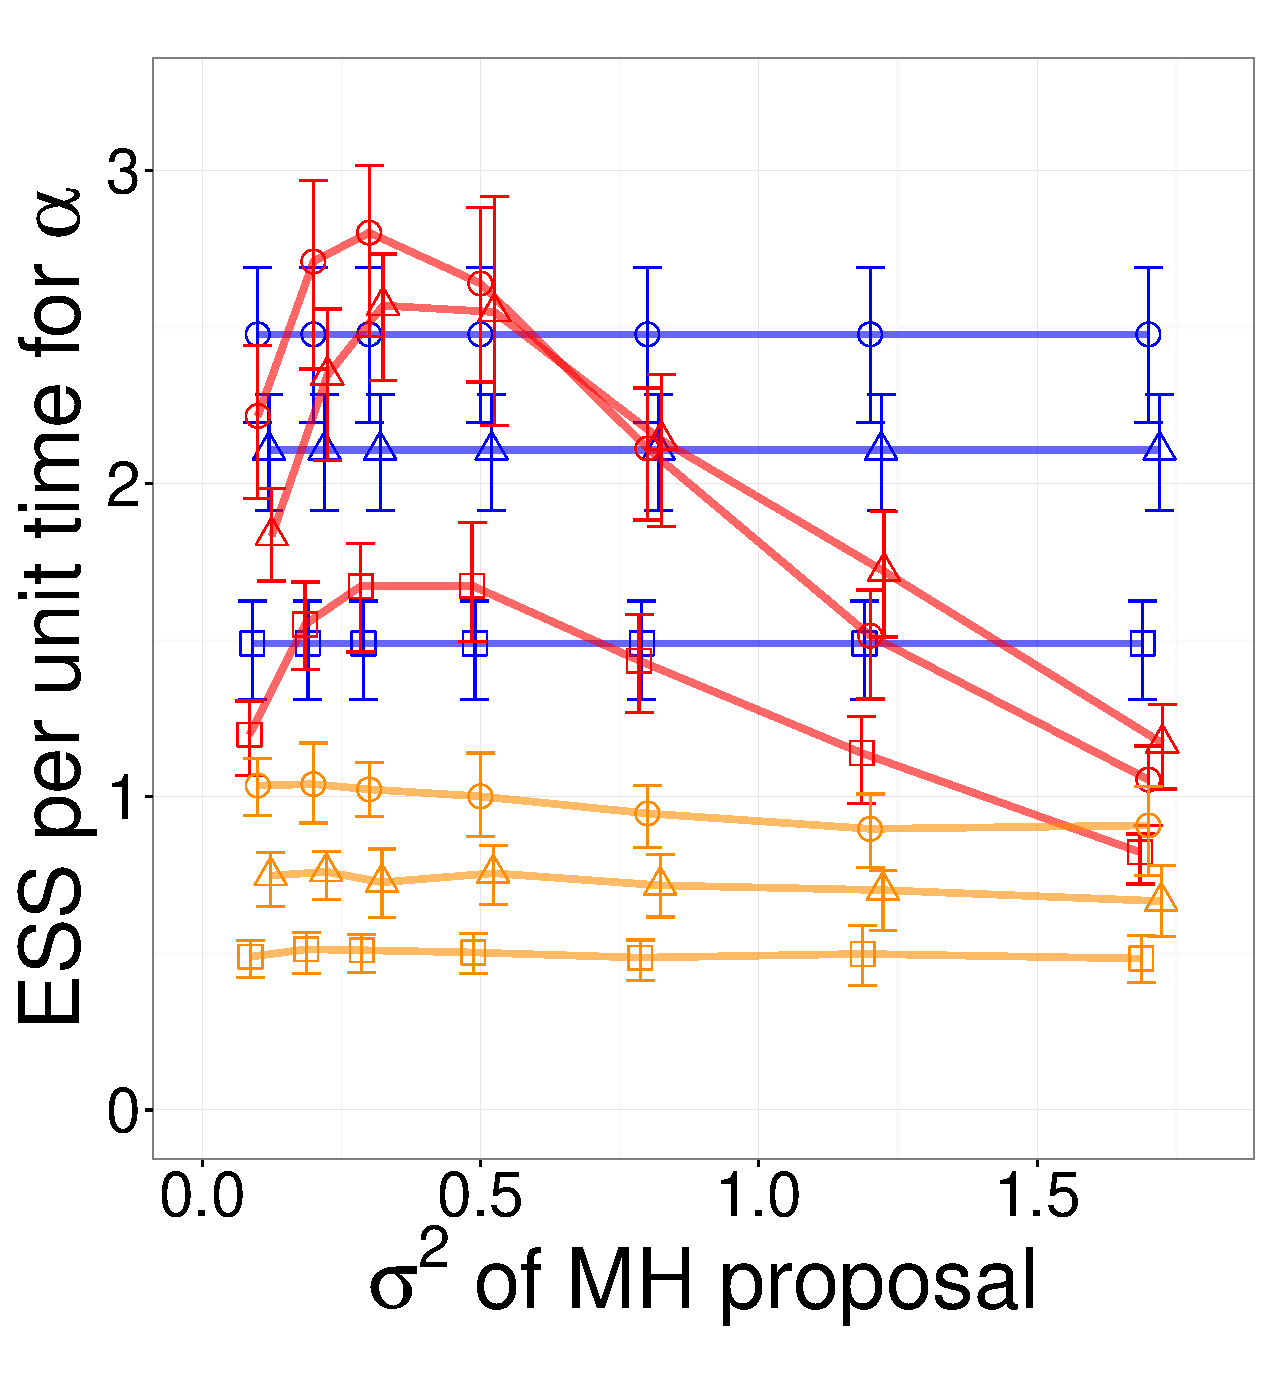
\includegraphics [width=0.90\textwidth, angle=0]{figs/q_5_alpha.pdf}
      \end{minipage}
  \begin{minipage}[hp]{0.45\linewidth}
  \centering
    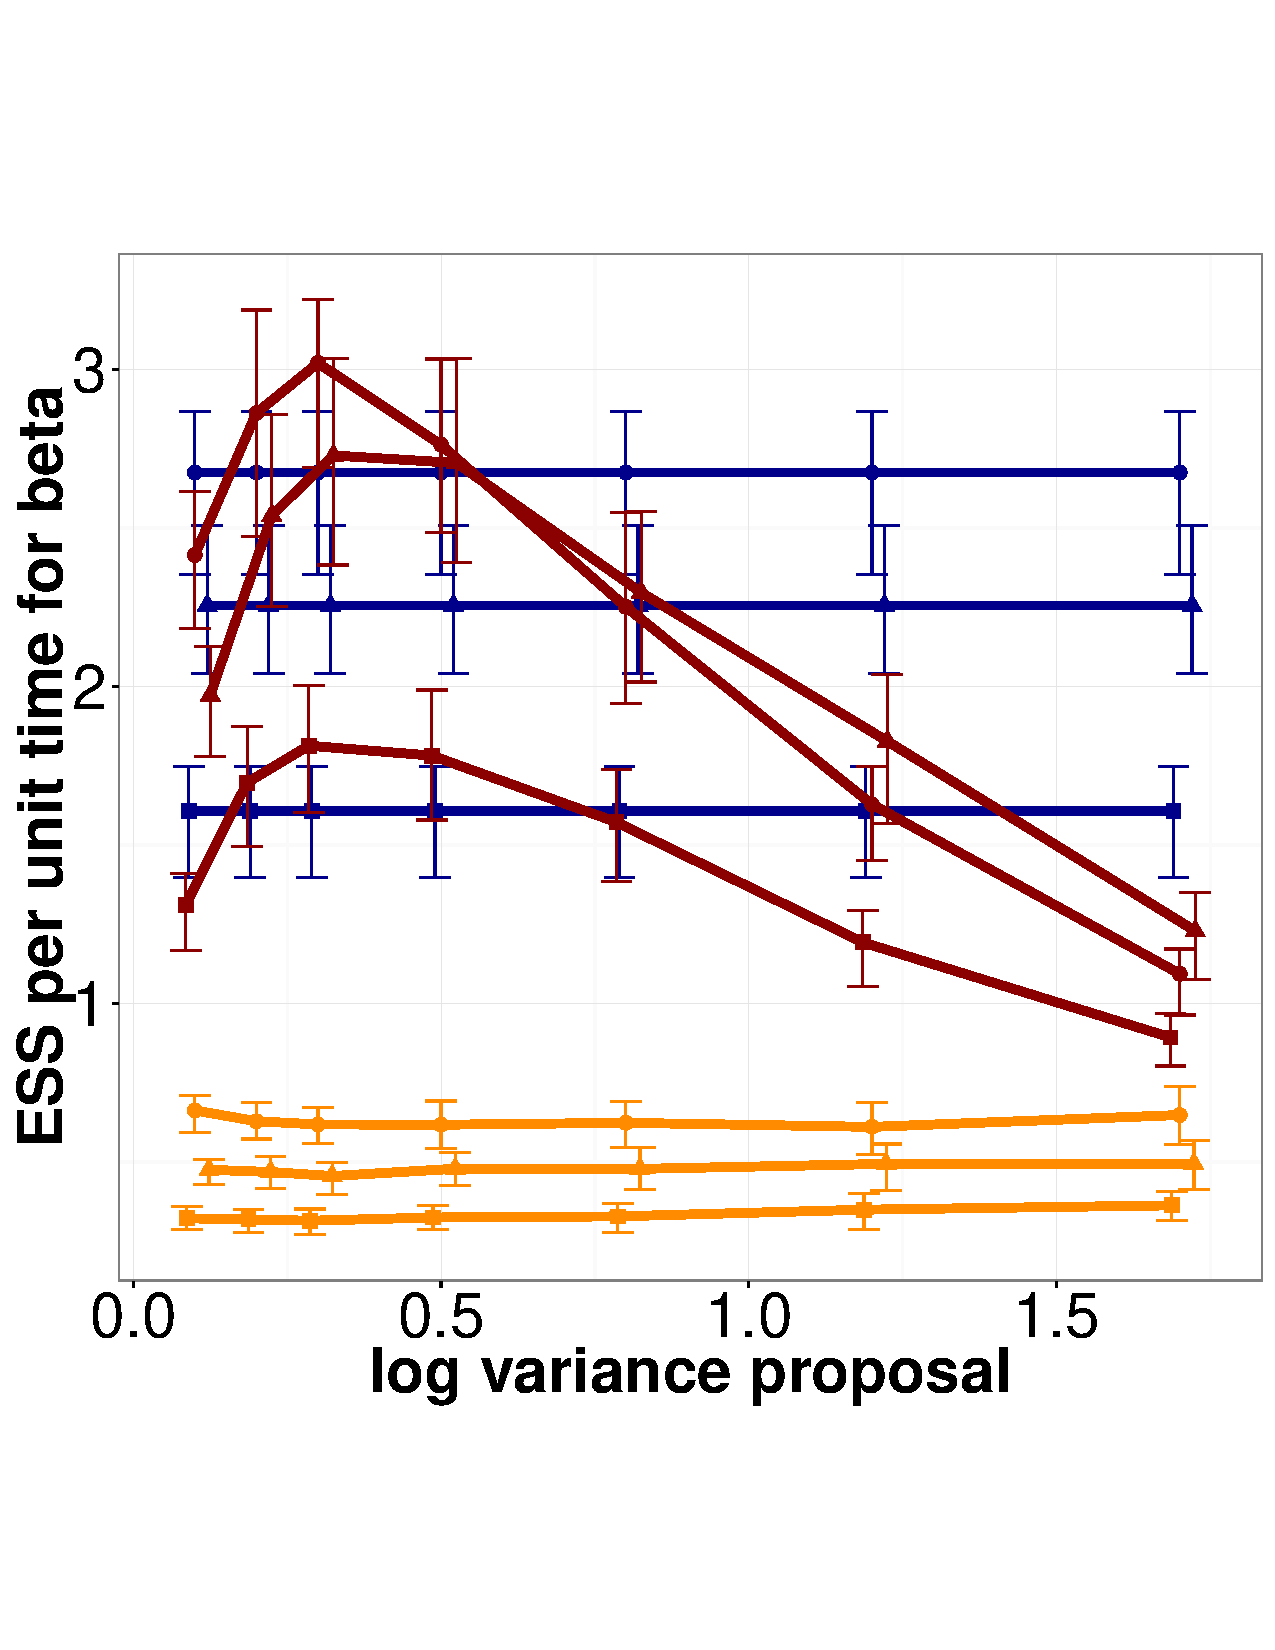
\includegraphics [width=0.90\textwidth, angle=0]{figs/q_5_beta.pdf}
    \vspace{-0 in}
      \label{fig:ESS_Q_D5}
  \end{minipage}
    \caption{ESS/sec for Immigration model (dim 5).The left is for $\alpha$, and the right is for $\beta$.}
  \end{figure}

\section{Non-homogeneous immigration model}

  \begin{figure}%[b]
  \centering
  \begin{minipage}[!hp]{0.45\linewidth}
  \centering
    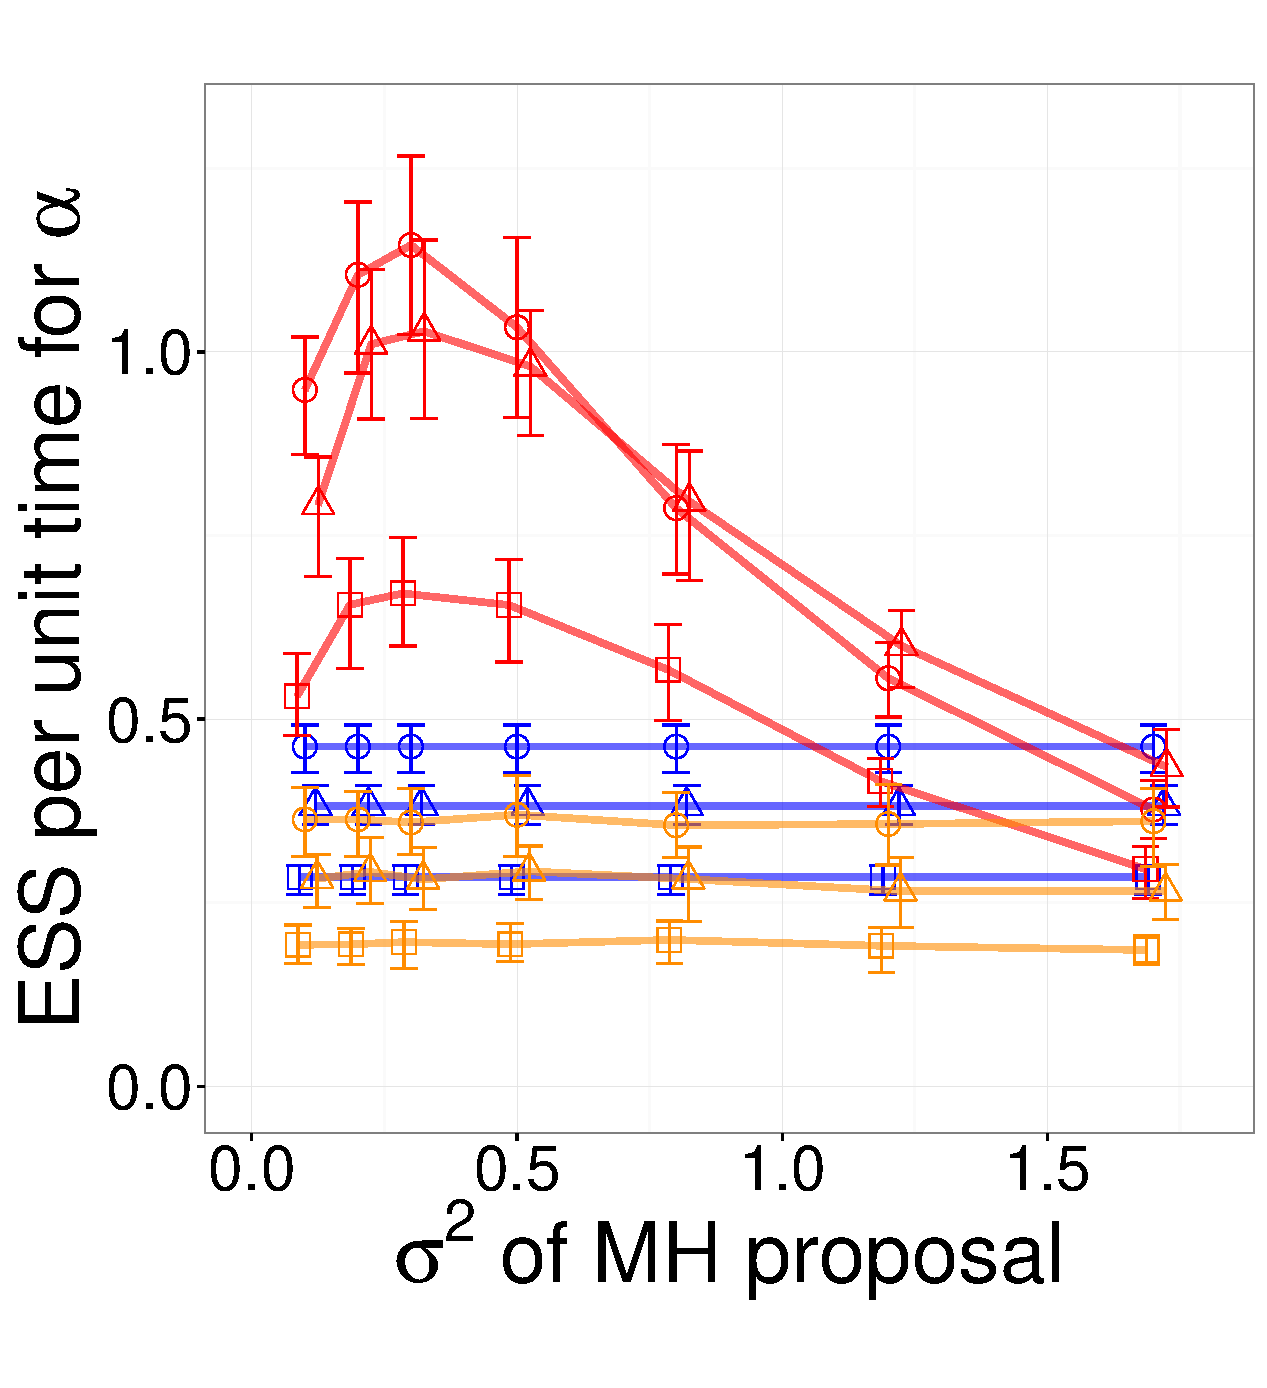
\includegraphics [width=0.70\textwidth, angle=0]{figs/pc_5_alpha.pdf}
      \end{minipage}
  \begin{minipage}[!hp]{0.45\linewidth}
  \centering
    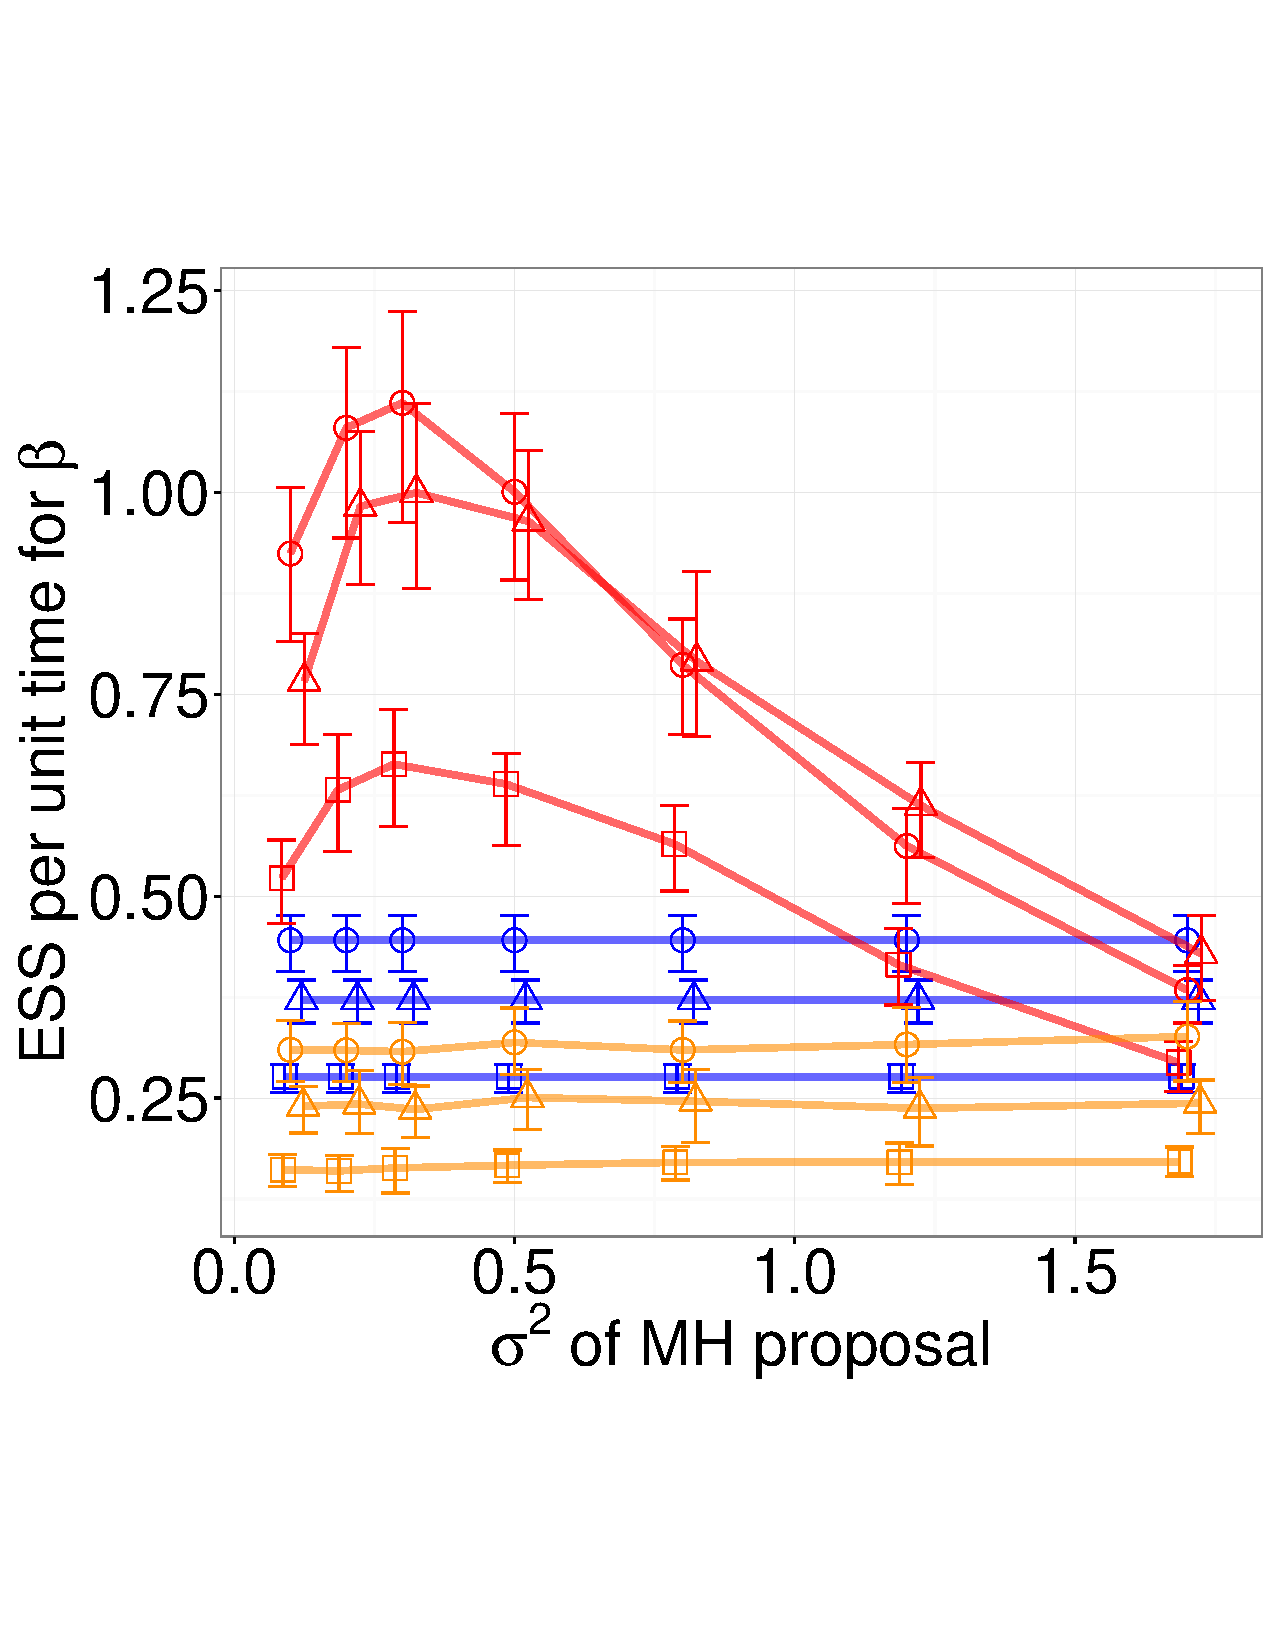
\includegraphics [width=0.70\textwidth, angle=0]{figs/pc_5_beta.pdf}
    \vspace{-0 in}
     \label{fig:ESS_pc_5}
  \end{minipage}
    \caption{ESS/sec for NH Immigration model (dim 5)}
  \end{figure}

  \subsection{Immigration models with capacity}
\noindent Assume: $S = [S_0,S_1, ...,S_N] \;, T = [t_0(t_{start}), t_1,...,t_N, t_{N+1}(t_{end})]$, and y as observations.\\
Now, let's consider a immigration model as follows. State space is $\{0, 1, 2, ..., N - 1\}$, representing the total population. The transition matrix is defined as follows. 
$$A_i =: A_{i,i} = -(\alpha + i\beta), \; \; i =0,1,...,N$$ $$A_{i, i+1} = \alpha, \; \; i =0,1,...,N-1,$$ $$A_{i, i-1}  = \beta, \; \;  i =1,...,N.$$
We already know the conditional density(given $\alpha,\; \beta$) of a MJP trajectory $(s_0, S, T)$ in time interval $[t_{start}, t_{end}]$, with $S=(s_1, s_2,..., s_k)$, $T=(t_1, t_2,..., t_k)$. 
$$f(s_0,S,T| \alpha, \beta) = \prod_{i=0}^{k-1} A_{s_i, s_{i+1}} \exp(\sum_{i=0}^{k} A_{s_i}(t_{i+1} - t_{i})), $$
where $t_0 = t_{start}$, $t_{k+1} = t_{end}.$\\
Let's denote some notations here.\\
$$U(s_0, S, T):= \sum_{i=0}^{k-1} \mathbb{I}_{\{s_{i+1} - s_i = 1\}}.$$
$$D(s_0, S, T):= \sum_{i=0}^{k-1} \mathbb{I}_{\{s_{i+1} - s_i = -1\}}.$$
Call them U and D for short.
Let's denote the total time when the trajectory state stays at state i as $\tau_i$, i.e. $\tau_i = \sum_{j=0}^{k} (t_{j+1} -t_j)\mathbb{I}_{\{s_j = i\}}$, then $\sum_{i=0}^k (t_{i+1} - t_i)s_i = \sum_{i=0}^N \tau_ii.$\\

$$f(s_0,S,T| \alpha, \beta) = \exp(-\alpha(t_{end} - t_{start}- \tau_N) )\alpha^U \cdot  \exp((-(\sum_{i=0}^k (t_{i+1} - t_i)s_i)\beta) \prod_{i=1}^N i^{\sum_{j=0}^{k-1}\mathbb{I}_{s_{j+1} = i -1 \;,  s_j = i} }   \beta^D$$\\
If we assume the prior of $\alpha$, and $\beta$ are $Gamma(\mu,\lambda)$, $Gamma(\omega, \theta)$, which are independent with each other. \\
$$p(\alpha) = \frac{\lambda^\mu}{\Gamma(\mu)}\alpha^{\mu -1}e^{-\lambda \alpha}. $$
$$p(\beta) = \frac{\theta^\omega}{\Gamma(\omega)}\beta^{\omega -1}e^{-\theta \beta}. $$
Then we can get the posterior distribution $$f(\alpha, \beta | s_0,S,T)$$ as follows.
$$ f(\alpha, \beta | s_0,S,T) \propto \exp(-(\lambda + t_{end} - t_{start}- \tau_N)\alpha) \alpha^{\mu + U -1} \cdot \exp(-(\sum_{i=0}^k (t_{i+1} - t_i)s_i + \theta)\beta) \beta^{\omega+ D -1}.$$
It means that the posterior distributions of $\alpha$, $\beta$ are still independent. \\
$\alpha | s_0,S,T$ is following $Gamma(\mu+ U,\lambda + t_{end} - t_{start}- \tau_N)$\\
$\beta | s_0,S,T$ is following $Gamma(\omega+ D,\theta + \sum_{i=0}^k (t_{i+1} - t_i)s_i)$, which is equivalent to $Gamma(\omega+ D,\theta +\sum_{i=0}^N \tau_ii)$\\
Such immigration models have perfectly conjugate posterior distributions when we assign $\gamma$ priors to $\alpha$ and $\beta$. We apply our Metropolis Hasting algorithms on such models to compare the performance with the performance of Gibbs Sampling algorithm.
